\section{Auswertung}
\subsection{Mittlere freie Weglänge}
Der Dampfdruck $p_\text{sät}$ und die mittlere freie Weglänge $\bar{w}$ ergeben sich aus der verwendeten Temperatur \ref{eqn:weglaenge} (siehe Tab. \ref{tab:weglaenge}).
Der Abstand $a$ zwischen Kathode und Beschleunigungselektrode beträgt $\SI{1}{\centi\metre}$.
Das Verhältnis $\frac{\bar{w}}{a}$ soll $1000 - 4000$ kleiner als $a$ sein, damit eine ausreichende Stoßwahrscheinlichkeit gegeben ist.
\begin{table}
    \centering
    \begin{tabular}{cccc}
        \toprule
        Temperatur $\,/\, \si{\kelvin}$ & $p_\text{sät} \,/\, \si{\milli\bar}$ & $\bar{w} \,/\, \si{cm}$ & $\frac{a}{\bar{w}}$ \\
        \midrule
        $300.65$ & $0.0064$ & $0.45$ & $2.22$ \\
        $413.15$ & $3.25$ & $8.91 \cdot 10^{-4}$ & $1122.33$ \\
        $453.15$ & $14.14$ & $2.05 \cdot 10^{-4}$ & $4876.12$ \\
        \bottomrule
    \end{tabular}
    \caption{Der Sättigungsdampfdruck $p_\text{sät}$, die mittlere freie Weglänge $\bar{w}$ und das Verhältnis $\frac{a}{\bar{w}}$ für die Gefäßtemperatur $T$.}
    \label{tab:weglaenge}
\end{table}

\FloatBarrier
\subsection{Integrale Energieverteilung}
In Tab. \ref{tab:messwerte_raumtemperatur} befinden sich die gemessenen Werte bei Raumtemperatur ($T=\SI{300.65}{\kelvin}$) und in Tab. \ref{tab:messwerte_140} die Messwerte bei einer Gefäßtemperatur $T=\SI{413.15}{\kelvin}$.
Die Beschleunigungsspannung wird konstant bei $U_B = \SI{11}{\volt}$ gehalten.
\begin{table}
    \centering
    \csvreader[tabular=cc,
    head=false,
    table head= $U_A \,/\, \si{\volt}$ & $I_A \,/\, \si{\nano \ampere}$ \\
    \midrule,
    late after line= \\]
    {content/data/raumtemperatur.csv}{1=\eins, 2=\zwei}{$\num{\eins}$ & $\num{\zwei}$}
    \caption{Der gemessene Auffängerstrom $I_A$ in Abhängigkeit der Bremsspannung $U_A$ bei konstanter Beschleunigungsspannung $U_B = \SI{11}{\volt}$ und Temperatur $T = \SI{300.65}{\kelvin}$.}
    \label{tab:messwerte_raumtemperatur}  
\end{table}

\begin{table}
    \centering
    \csvreader[tabular=cc,
    head=false,
    table head= $U_A \,/\, \si{\volt}$ & $I_A \,/\, \si{\nano \ampere}$ \\
    \midrule,
    late after line= \\]
    {content/data/140_grad.csv}{1=\eins, 2=\zwei}{$\num{\eins}$ & $\num{\zwei}$}
    \caption{Der gemessene Auffängerstrom $I_A$ in Abhängigkeit der Bremsspannung $U_A$ bei konstanter Beschleunigungsspannung $U_B = \SI{11}{\volt}$ und Temperatur $T = \SI{413.15}{\kelvin}$.}
    \label{tab:messwerte_140}  
\end{table}
\FloatBarrier
Der gemessene Auffängerstrom $I_A$ bei Raumtemperatur ($T = \SI{27.5}{\degreeCelsius}$) ist in Abb. \ref{fig:raumtemperatur_int} graphisch dargestellt.
Die Messwerte für $T = \SI{140}{\degreeCelsius}$ sind in Abb. \ref{fig:140_int} zu sehen.

\begin{figure}
    \centering
    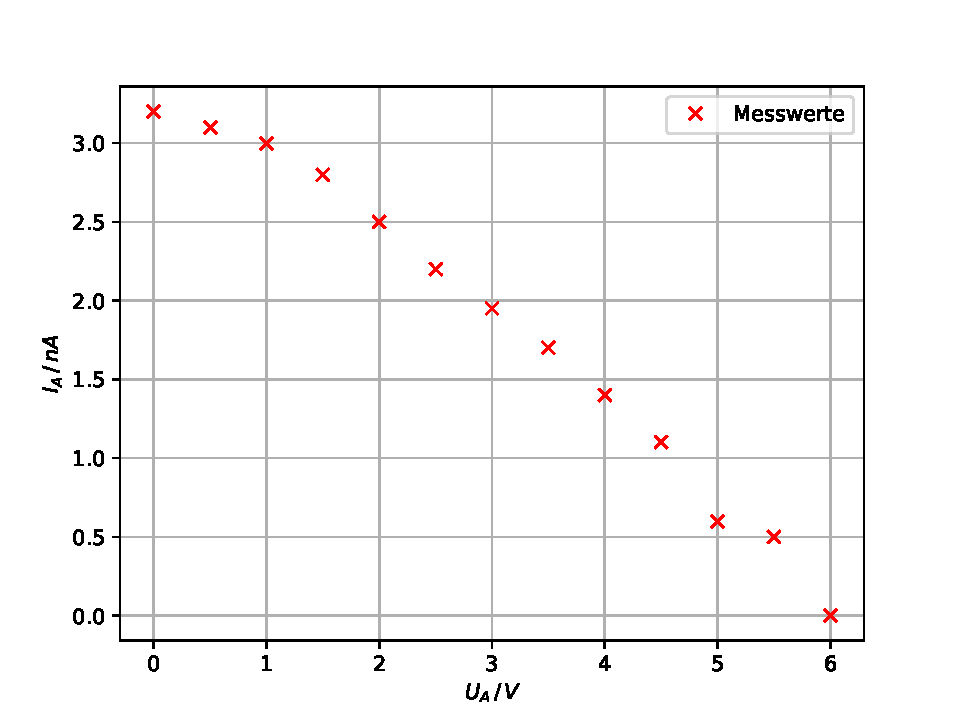
\includegraphics[width=0.8\textwidth]{content/data/raumtemperatur_int.pdf}
    \caption{Integrale Energieverteilung für $T=\SI{27.5}{\degreeCelsius}$. \cite{matplotlib}\cite{numpy}}
    \label{fig:raumtemperatur_int}
\end{figure}

\begin{figure}
    \centering
    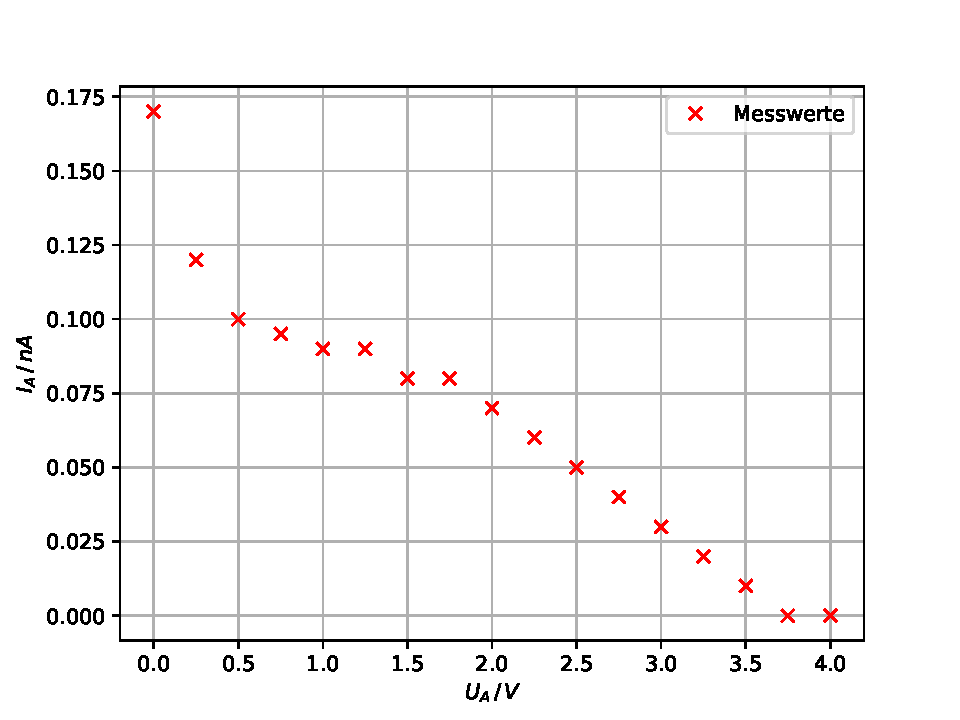
\includegraphics[width=0.8\textwidth]{content/data/140_int.pdf}
    \caption{Integrale Energieverteilung für $T=\SI{140}{\degreeCelsius}$. \cite{matplotlib}\cite{numpy}}
    \label{fig:140_int}
\end{figure}

\FloatBarrier
\subsection{Differentielle Energieverteilung}
Die differentielle Energieverteilung ergibt sich aus der Steigung der integralen Energieverteilung:
\begin{align*}
    \text{Steigung} &= \frac{\Delta I_A}{\Delta U_A} \\
    &= \frac{I_{A,k} - I_{A,k-1}}{U_{A,k} - U_{A,k-1}}
\end{align*}
Die Steigung der integralen Energieverteilung ist in Tab. \ref{tab:raumtemperatur_dif} für $T=\SI{27.5}{\degreeCelsius}$ und in Tab. \ref{tab:140_grad_dif} für $T=\SI{140}{\degreeCelsius}$ aufgelistet.
\begin{table}
    \centering
    \begin{tabular}{cc}
        \toprule
        $U_A \,/\, \si{\volt}$ & $|\frac{\Delta I_A}{\Delta U_A}| \,/\, \si{\frac{\nano\ampere}{\volt}}$ \\
        \midrule
        $0.0$ & $0.2$\\
        $0.5$ & $0.2$\\
        $1.0$ & $0.4$\\
        $1.5$ & $0.6$\\
        $2.0$ & $0.6$\\
        $2.5$ & $0.5$\\
        $3.0$ & $0.5$\\
        $3.5$ & $0.6$\\
        $4.0$ & $0.6$\\
        $4.5$ & $1.0$\\
        $5.0$ & $0.2$\\
        $5.5$ & $1.0$\\
        \bottomrule
    \end{tabular}
    \caption{Die differentielle Energieverteilung für $T=\SI{27.5}{\degreeCelsius}$.}
    \label{tab:raumtemperatur_dif}
\end{table}

\begin{table}
    \centering
    \begin{tabular}{cc}
        \toprule
        $U_A \,/\, \si{\volt}$ & $|\frac{\Delta I_A}{\Delta U_A}| \,/\, \si{\frac{\pico\ampere}{\volt}}$ \\
        \midrule
        $0.00$ & $200$ \\ 
        $0.25$ & $80$ \\ 
        $0.50$ & $20$ \\ 
        $0.75$ & $20$ \\ 
        $1.00$ & $0$ \\ 
        $1.25$ & $40$ \\ 
        $1.50$ & $0$ \\ 
        $1.75$ & $40$ \\ 
        $2.00$ & $40$ \\ 
        $2.25$ & $40$ \\ 
        $2.50$ & $40$ \\ 
        $2.75$ & $40$ \\ 
        $3.00$ & $40$ \\ 
        $3.25$ & $40$ \\ 
        $3.50$ & $40$ \\ 
        $3.75$ & $0$ \\
        \bottomrule
    \end{tabular}
    \caption{Die differentielle Energieverteilung für $T=\SI{140}{\degreeCelsius}$.}
    \label{tab:140_grad_dif}
\end{table}
Die differentielle Energieverteilung ist in Abb. \ref{fig:raumtemperatur_dif} und \ref{fig:140_grad_dif} dargestellt.
\begin{figure}
    \centering
    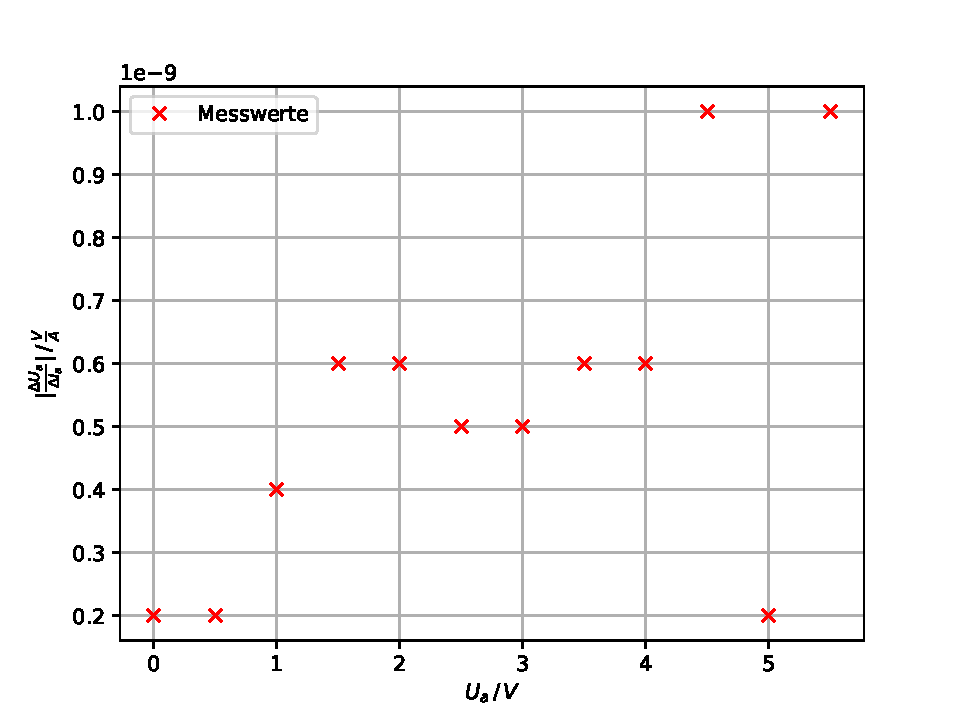
\includegraphics[width=0.8\textwidth]{content/data/raumtemperatur_dif.pdf}
    \caption{Die differentielle Energieverteilung für $\SI{27.5}{\degreeCelsius}$ graphisch dargestellt. \cite{matplotlib}\cite{numpy}}
    \label{fig:raumtemperatur_dif}
\end{figure}
\begin{figure}
    \centering
    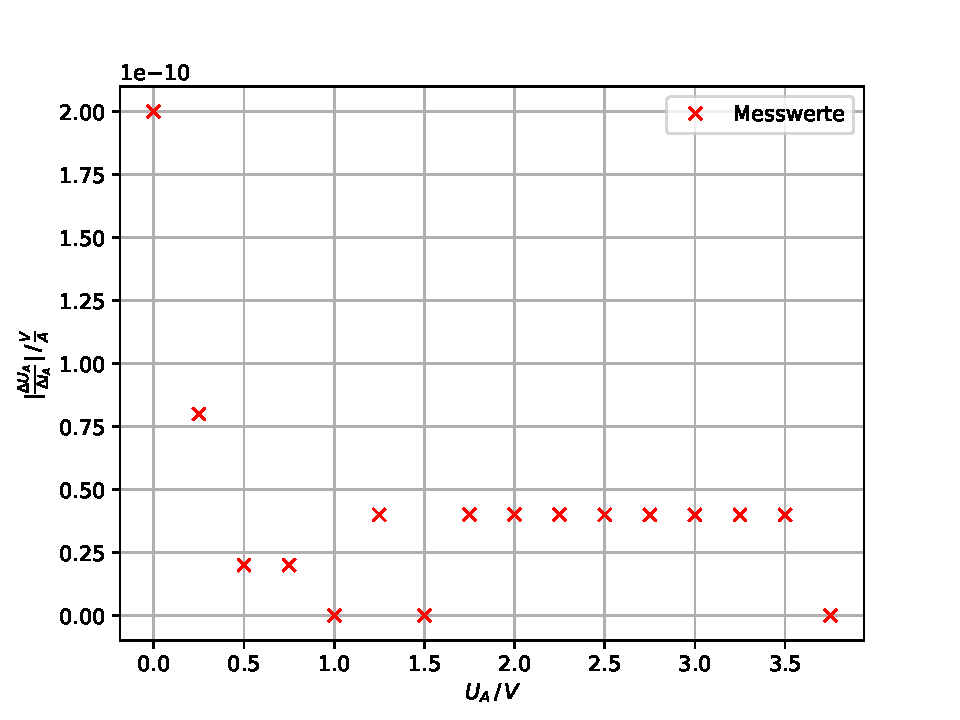
\includegraphics[width=0.8\textwidth]{content/data/140_grad_dif.pdf}
    \caption{Die differentielle Energieverteilung für $\SI{140}{\degreeCelsius}$ graphisch dargestellt. \cite{matplotlib}\cite{numpy}}
    \label{fig:140_grad_dif}
\end{figure}
\FloatBarrier

\subsection{Franck-Hertz-Kurve}
Als nächstes wird das Gegenpotential konstant auf $U_A = \SI{1}{\volt}$ und die Temperatur auf $T = \SI{180}{\degreeCelsius}$ eingestellt.
Die Beschleunigungsspannung $U_B$ wird im Intervall von $\SI{0}{\volt}$ bis $\SI{60}{\volt}$ in $\Delta U_B = \SI{1}{\volt}$-Schritten varriert und der Auffängerstrom $I_A$ gemessen.
Die Messwerte in Tab. \ref{tab:franck_hertz} sind in Abb. \ref{fig:franck_hertz} graphisch dargestellt und die Maxima visuell hervorgehoben.
\begin{table}
    \centering
    \begin{tabular}{cc|}
        \toprule
        $U_B \,/\, \si{\volt}$ & $I_A \,/\, \si{\nano\ampere}$ \\
        \midrule
        $0$ & $0.00$ \\
        $1$ & $0.00$ \\
        $2$ & $0.00$ \\
        $3$ & $0.00$ \\
        $4$ & $0.00$ \\
        $5$ & $0.00$ \\
        $6$ & $0.00$ \\
        $7$ & $0.00$ \\
        $8$ & $0.00$ \\
        $9$ & $0.00$ \\
        $10$ & $0.00$ \\
        $11$ & $0.00$ \\
        $12$ & $0.00$ \\
        $13$ & $0.00$ \\
        $14$ & $0.00$ \\
        $15$ & $0.01$ \\
        $16$ & $0.00$ \\
        $17$ & $0.00$ \\
        $18$ & $0.00$ \\
        $19$ & $0.01$ \\
        $20$ & $0.05$ \\
        $21$ & $0.00$ \\
        $22$ & $0.00$ \\
        $23$ & $0.00$ \\
        $24$ & $0.03$ \\
        $25$ & $0.09$ \\
        $26$ & $0.05$ \\
        $27$ & $0.00$ \\
        $28$ & $0.00$ \\
        $29$ & $0.05$ \\
        $30$ & $0.14$ \\
        \bottomrule
    \end{tabular}
        \begin{tabular}{|cc}
        \toprule
        $U_B \,/\, \si{\volt}$ & $I_A \,/\, \si{\nano\ampere}$ \\
        \midrule
        $31$ & $0.12$ \\
        $32$ & $0.02$ \\
        $33$ & $0.02$ \\
        $34$ & $0.08$ \\
        $35$ & $0.18$ \\
        $36$ & $0.22$ \\
        $37$ & $0.11$ \\
        $38$ & $0.06$ \\
        $39$ & $0.11$ \\
        $40$ & $0.25$ \\
        $41$ & $0.34$ \\
        $42$ & $0.26$ \\
        $43$ & $0.18$ \\
        $44$ & $0.20$ \\
        $45$ & $0.34$ \\
        $46$ & $0.47$ \\
        $47$ & $0.44$ \\
        $48$ & $0.35$ \\
        $49$ & $0.32$ \\
        $50$ & $0.42$ \\
        $51$ & $0.60$ \\
        $52$ & $0.65$ \\
        $53$ & $0.60$ \\
        $54$ & $0.58$ \\
        $55$ & $0.68$ \\
        $56$ & $0.88$ \\
        $57$ & $0.99$ \\
        $58$ & $1.05$ \\
        $59$ & $1.10$ \\
        $60$ & $1.20$ \\
             &        \\
        \bottomrule
    \end{tabular}
    \caption{Messwerte zur Franck-Hertz-Kurve bei einer Temperatur von $T = \SI{180}{\degreeCelsius}$ und einem Gegenpotential von $U_A = \SI{1}{\volt}$. \cite{matplotlib}\cite{scipy}\cite{uncertainties}\cite{numpy}}
    \label{tab:franck_hertz}
\end{table}

\begin{figure}
    \centering
    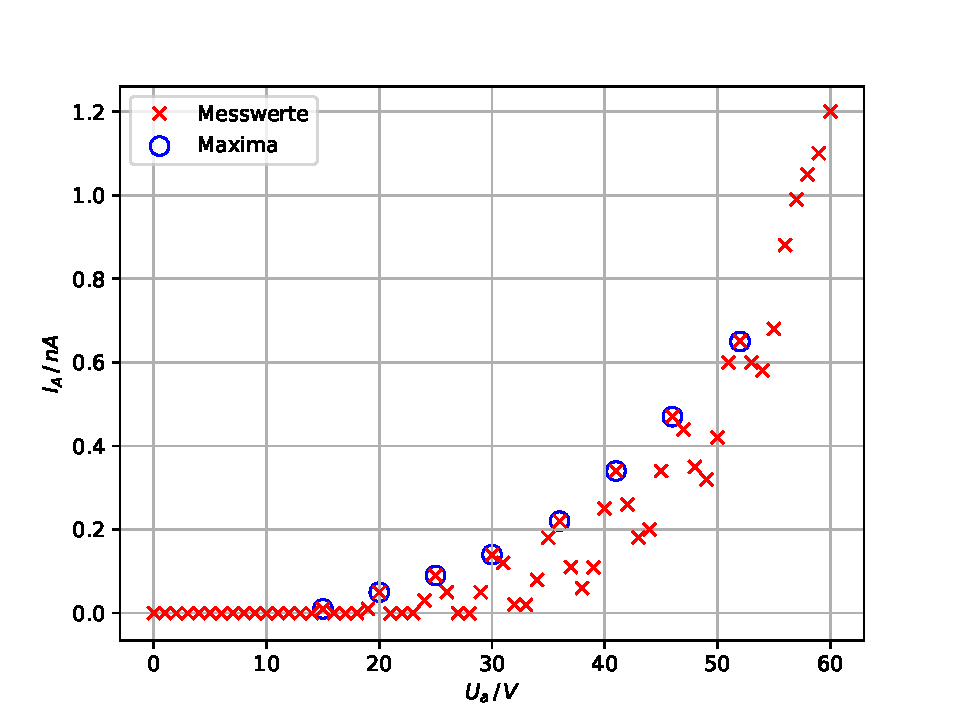
\includegraphics[width=0.8\textwidth]{content/data/franck_hertz.pdf}
    \caption{Franck-Hertz-Kurve bei einer Temperatur von $T = \SI{180}{\degreeCelsius}$ und einem Gegenpotential von $U_A = \SI{1}{\volt}$. \cite{matplotlib}\cite{scipy}\cite{uncertainties}\cite{numpy}}
    \label{fig:franck_hertz}
\end{figure}

\FloatBarrier
Die Abstände der Maxima werden mithilfe der Bibliotheken Numpy\cite{numpy} und scipy\cite{scipy} bestimmt und sind in Tab. \ref{tab:abstand} aufgelistet.
\begin{table}
    \centering
    \begin{tabular}{ccc}
        \toprule
        $U_{B,max} \,/\, \si{\volt}$ & $I_{A,max} \,/\, \si{\nano\ampere}$ & $\Delta U_{B,max} \,/\, \si{\volt} $ \\
        \midrule
        $15$ & $0.01$ & $5$ \\
        $20$ & $0.05$ & $5$ \\
        $25$ & $0.09$ & $5$ \\
        $30$ & $0.14$ & $6$ \\
        $36$ & $0.22$ & $5$ \\
        $41$ & $0.34$ & $5$ \\
        $46$ & $0.47$ & $6$ \\
        $52$ & $0.65$ & - \\
        \bottomrule
    \end{tabular}
    \caption{Maxima und Abstände der Maxima der Franck-Hertz-Kurve. Abstand bezeichnet hier den Abstand zum nächsten Maximum.}
    \label{tab:abstand}
\end{table}
Im Mittel ergibt sich ein Abstand von
\begin{equation*}
    \Delta \bar{U}_{B,max} = \SI{5.29(18)}{\volt}
\end{equation*}
und somit eine Anregungsenergie für den 1. Zustand von Quecksilber von
\begin{equation}
    U_1 = \SI{5.29(18)}{\electronvolt} \, .
\end{equation}
Aus der 1. Anregungsenergie folgt die Wellenlänge der beim Übergang in den Grundzustand emittierten Strahlung
\begin{align*}
    \lambda &= \frac{h \cdot c}{U_1} \\
    &= \SI{235(8)}{\nano\metre} \, .
\end{align*}
Das 1. Maximum liegt bei $U_{B,max}=\SI{15}{\volt}$ und es gilt $U_{B,max} = K + U_1$.
Daraus folgt sofort für das Kontaktpotential
\begin{equation}
    K = \SI{9.71(18)}{\volt} \, .
\end{equation}